 
\chapter{Discontinuous solutions of hyperbolic systems-shocks}\label{chap3}

\section{Introduction}\label{chap3:sec3.1}

We\pageoriginale illustrate the notion of a solution with shocks via a
very simple equation known as the Burger's equation. We derive the
Rankine-Hugoniot relation to determine the curve across which a
discontinuity occurs. We then generalise these ideas to a system of
equations.

\section{Burger's equation}\label{chap3:sec3.2}

Burger's equation is given by
\begin{equation*}
\frac{\partial u}{\partial t} + u \frac{\partial u}{\partial x} = 0. 
\tag{3.1}\label{eq3.1}
\end{equation*}
(In the literature one also finds at times an extra term $-\epsilon
\dfrac{\partial^2 u}{\partial x^2}$ on the left hand side, but we
consider the limiting case as $\epsilon \to 0$). This equation is
trivially a hyperbolic ``system'' (a system with a matrix of order 1
and the single eigen value $u!$). If we set
\begin{equation*}
\frac{dt}{ds} = 1; \; \frac{dx}{dt} = u(x,t), \tag{3.2}\label{eq3.2}
\end{equation*}
then (\ref{eq3.1}) will read as 
\begin{equation*}
\frac{du}{ds} = \frac{\partial u}{\partial t} \frac{dt}{ds} +
\frac{\partial u}{\partial x} \frac{dx}{ds} = 0. \tag{3.3}\label{eq3.3}
\end{equation*}
Hence $u$ is constant along the characteristic curve $C$ whose slope
is given by 
\begin{equation*}
\frac{dx}{dt} = u (x,t). \tag{3.4}\label{eq3.4}
\end{equation*}
Thus from (\ref{eq3.4}) and the fact that $u$ is constant along $C$ we see
that all the characteristics of (\ref{eq3.1}) are straight lines.

In the following figure, the lower graph indicates the initial value
$u(x,0)$ as a function of $x$. The characteristics through $(x, 0)$
in the $x-t$ plane are shown in the upper graph. These are lines whose
slopes are given by (\ref{eq3.4}).
 
\begin{figure}[H]
\centering
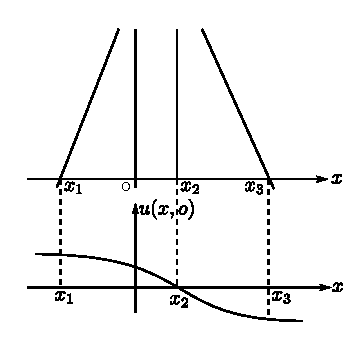
\includegraphics{figures/fig52-3.1.eps}
\caption{}\label{c3:fig3.1}
\end{figure}\pageoriginale

(Since $u(x_1, 0) > 0$, the characteristic at $(x_1, 0)$ has
positive slope and so on).

Note, however, that for an arbitrary initial value function
$u(x,0)$, it is possible that the various characteristics
intersect. Then we have a contrdiction because the point of
intersection lies on two different characteristics and must possess
two different values of $u$, which is impossible.

So we try to find a discontinuous solution to this problem. For this
we need the notion of the weak form of the equation.

To do this we first rewrite the equation (\ref{eq3.1}) in the {\em proper}
conservative form:
\begin{equation*}
\frac{\partial u}{\partial t} + \frac{\partial}{\partial x}
\left(\frac{1}{2} u^2\right) = 0. 
\tag{3.5}\label{eq3.5}
\end{equation*}
(The\pageoriginale importance of the proper conservative form cannot
be over-\break emphasized. Cf. Remark \ref{chap3:rem3.2}).

Let $\varphi$ be a test-function (i.e. a function over $\mathbb{R}_x
\times \mathbb{R}_t$ with compact support which is as smooth as we
please). We multiply (\ref{eq3.5}) by $\varphi$ and integrate by parts over
the domain $\Omega$, where 
$$
\Omega = \mathbb{R}_x \times \{t \in \mathbb{R} \mid t > 0\}.
$$
Thus we get
\begin{align*}
0 & = -\int_{\Omega} \varphi \left[\frac{\partial u}{\partial t} +
  \frac{\partial}{\partial x} \left(\frac{1}{2} u^2\right) \right] dx \; dt\\
& = \int_\Omega u\frac{\partial \varphi}{\partial t} dx\; dt +
\int^\infty_{-\infty} u (x,0) \varphi(x,0) dx + \int_\Omega
\frac{u^2}{2} \frac{\partial \varphi}{\partial x} dx \; dt
\end{align*}
where $u(x,0)$ is given to us already. The weak form is then the
problem of finding $u$ such that 
\begin{equation*}
\int_\Omega u\frac{\partial \varphi}{\partial t } dx \; dt +
\int_\Omega \frac{u^2}{2} \frac{\partial \varphi}{\partial x} dx \; dt
+ \int^\infty_{-\infty} u(x,0) \varphi(x,0) dx = 0
\tag{3.6}\label{eq3.6}  
\end{equation*}
for any test-function $\varphi$.

Note that if $u$ is smooth and satisfies (\ref{eq3.6}) we can reverse the
integration by parts and show that $u$ satisfies (\ref{eq3.5}) as well.

Let us now assume that $u$ is piecewise continuously
differentiable. Let $\Gamma$ be a curve across which a discontinuity
occurs in $u$. Assume that $\Gamma$ is smooth. Let $\Gamma$ divide the
domain $\Omega$ into two parts $\Omega_1$ and $\Omega_2$. Denote by
$\bar{n} = (n_x, n_t)$ the unit normal along $\Gamma$ directed from
$\Omega_1$ into $\Omega_2$. Thus $u\mid \Omega_i$ is smooth $(i=1,2)$
and $u$ satisfies (\ref{eq3.6}). By choosing $\varphi$ to have support
completely contained either in $\Omega_1$ or in $\Omega_2$ we see
immediately that $u\mid \Omega_i$ satisfies (\ref{eq3.5}) in $\Omega_i
(i=1,2)$. 

Now\pageoriginale choose $\varphi$ so that supp $\varphi \subset
\Omega$, and supp $\varphi \cap \Gamma$ is non-empty. We set down the
following notations:
\begin{equation*}
\left. 
\begin{aligned}
D_i & = \text{ supp. } \varphi \cap \Omega_i, \; i = 1,2.\\
F & = \text{ supp } \varphi \cap \Gamma.
\end{aligned}
\right\}
\tag{3.7}\label{eq3.7}
\end{equation*}

\begin{figure}[H]
\centering
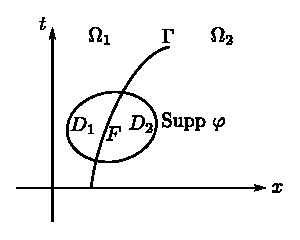
\includegraphics{figures/fig52-3.2.eps}
\caption{}\label{c3:fig3.2}
\end{figure}

Using this particular test-function $\varphi$ in (\ref{eq3.6}) and splitting
the integrals over $D_i(i=1,2)$, we get
\begin{align*}
0 & = \int_{D_1} \left(u\varphi_t + \frac{u^2}{2}\varphi_x\right) dx \; dt +
\int_{D_2} \left(u\varphi_t + \frac{u^2}{2}\varphi_x\right) dx \; dt\\
& = -\int_{D_1} {}^1 u_t \varphi dx \; dt + \int^{1}_F u \varphi n_t
ds - \int_{D_1} \left(\frac{({}_1 u)^2}{2}\right)_x \varphi dx\; dt\\ 
& \hspace{7cm} + \int_F \frac{({}^1 u)^2}{2} \varphi n_x dx\\
& \quad - \int_{D_2} {}^2 u_t \varphi dx \; dt - \int_F {}^2 u \varphi
n_t ds - \int_{D_2} \left(\frac{({}^2u)^2}{2}\right)_x \varphi dx \;
dt\\ 
& \hspace{7cm} - \int_F \frac{({}^2 u)^2}{2}  \varphi n_x ds
\end{align*}
where, $ds$ denotes integration along $F$, and ${}^1 u = u \mid
\Omega_1$, ${}^2 u = u\mid \Omega_2$. The change of sign in the
integrals over $F$ for the second set of terms is due to the fact that
the outer normal to $\Omega_2$ is the negative of the to
$\Omega_1$. Since ${}^1u$ and ${}^2u$ are smooth inside their domains,
they satisfy (\ref{eq3.5}) in these domains and hence\pageoriginale in the
above expression the integrals over $D_1$ and $D_2$ vanish. Thus we
are left with 
\begin{equation*}
\int_F \varphi \left[ ({}^1 u- {}^2 u) n_t + \left(\frac{({}^1u)^2}{2} -
  \frac{({}^2 u)^2}{2}\right) n_x\right] dx = 0 \tag{3.8}\label{eq3.8}
\end{equation*}
for all test-functions $\varphi$ with support in $\Omega$. Therefore
if we define the jump in a function $f$ across $\Gamma$ by
\begin{equation*}
[f] = {}^1 f - {}^2 f,
\tag{3.9}\label{eq3.9}
\end{equation*}
we then get
\begin{equation*}
[u] n_t + \left[\frac{u^2}{2}\right] n_x = 0. \tag{3.10}\label{eq3.10}
\end{equation*}
If we assume $\Gamma$ to be the curve $x = x(t)$, we can write
$\dfrac{dx}{dt} = \dfrac{-n_t}{n_x}$. Hence (\ref{eq3.10}) can be rewritten as 
\begin{equation*}
[u] \frac{dx}{dt} = \left[\frac{u^2}{2}\right].\tag{3.11}\label{eq3.11}
\end{equation*}

The relation (\ref{eq3.11}) is most fundamental in determining $\Gamma$. It is
known as the {\em Rankine-Hugoniot relation}.

We illustrate these ideas by means of examples.

\begin{exam}\label{chap3:exam3.1}
Let
$$
u(x,0) = 
\begin{cases}
1, & x \leq 0\\
0, & x > 0.
\end{cases}
$$
We then draw the characteristics as we did in Fig. \ref{c3:fig3.1}.

\begin{figure}[H]
\centering
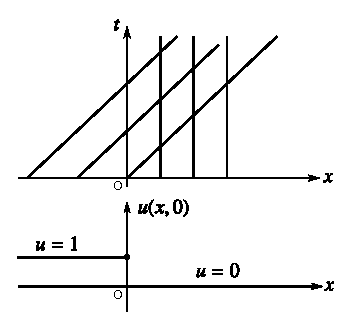
\includegraphics{figures/fig52-3.3.eps}
\caption{}\label{c3:fig3.3}
\end{figure}\pageoriginale

Thus we look for a discontinuous (weak) solution of the Burger's
equation which will be as in the following figure.

\begin{figure}[H]
\centering
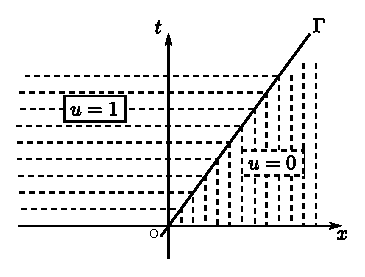
\includegraphics{figures/fig52-3.4.eps}
\caption{}\label{c3:fig3.4}
\end{figure}

The region shaded horizontally (to the left of $\Gamma$) has $u=1$ and
to the right of $\Gamma$ (shaded vertically) has $u=0$. 

To\pageoriginale determine the curve $\Gamma$ we use (\ref{eq3.11}). The jump
$[u] =1$ across $\Gamma$ and $\left[\dfrac{u^2}{2}\right] =
\frac{1}{2}$. Thus by (\ref{eq3.11}) one has
\begin{equation*}
\frac{dx}{dt} = \frac{1}{2}
\tag{3.12}\label{eq3.12}
\end{equation*}
as the slope of $\Gamma$. Thus $\Gamma$ is the straight line through
origin with slope given by (\ref{eq3.12}). 
\end{exam}

\begin{remark}\label{chap3:rem3.1}
This case has a parallel in the case of solution with shocks in fluid
dynamics. In gas dynamics, $\Gamma$ is the curve where the shock
occurs and $\dfrac{dx}{dt}$ is the speed of the shock. This speed is
`supersonic' (i.e. larger than the slopes of characteristics)
w.r.t. the state ahead and `subsonic' (i.e. smaller than the slope of
characteristics) w.r.t. the state behind. 
\end{remark}

\begin{exercise}\label{chap3:exer3.1}
Perform a similar analysis for the solution of the Burger's equation
when $u(x,0)$ is of the following form:
\begin{equation*}
u(x,0) = 
\begin{cases}
 1, & \text{ if } x \leq -1, \\
-x, & \text{ if } -1 \leq x \leq 0,\\
0, & \text{ if } x \geq 0.
\end{cases}
\end{equation*}
\end{exercise}

\begin{exam}\label{chap3:exam3.2}
Consider the solution of Burger's equation when the initial value is
given by 
$$
u(x,0) = 
\begin{cases}
0, & \text{ if } x < 0\\
1, & \text{ if } x \geq 0.
\end{cases}
$$
We then draw the characteristics. 
\begin{figure}[H]
\centering
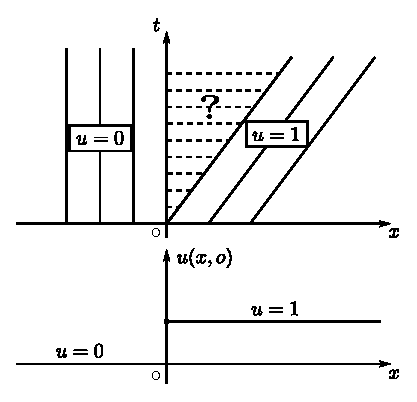
\includegraphics{figures/fig52-3.5.eps}
\caption{}\label{c3:fig3.5}
\end{figure}\pageoriginale

It is clear that in the region to the left of the $t$-axis (i.e. for
$x<0$) we must have $u(x,t) =0$. Similarly if $(x,t)$ lies to the
right of the line $x=t$ (i.e. the characteristic through the origin)
we must have $u(x,t) =1$. The problem is in the (shaded) region in
between. Here we now have two possibilities.

First we may search for a straight line $\Gamma$ passing throught
origin so that to its left, $u=0$ and to its right, $u=1$. Using
(\ref{eq3.11}) it is easy to check that this line has slope given by
$\dfrac{dx}{dt} = \frac{1}{2}$. 

On the other hand, we see that the function $x/t$ satisfies Burger's
equation. The solution tends to zero as $x \to 0$ and to 1 as $x \to
t$. Thus if we define $u$ to be $x/t$ in this region, we get a
continuous solution to Burger's equation. Thus we now have two
solutions to the equation (Cf. Fig. 3.6). 

\begin{figure}[H]
\centering
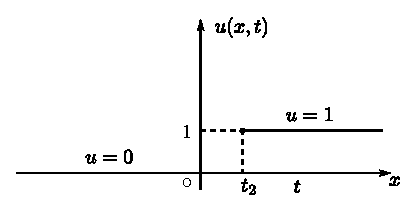
\includegraphics{figures/fig52-3.6a.eps}
\caption{(a): \textit{Discontinuous solution}}\label{c3:fig3.6}
\end{figure}
\pageoriginale 
\begin{figure}[H]
\centering
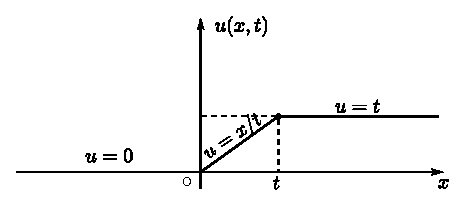
\includegraphics{figures/fig52-3.6b.eps}
\centerline{(b): \textit{Continuous solution}}
\end{figure}

We therefore need one more condition to fix up uniquely the solution
for Burger's equation in this case. Such a condition comes from
analogy with physical considereations of admissibility of a
solution. We demand that $\dfrac{\partial u}{\partial x} \neq +
\infty$. Using this we see that the {\em continuous} solution alone is
admissible. The ``velocity'' $u$ in case of a shock cannot step up in
the positive direction of the $x$-axis.

This latter example is the analogue of a rarefaction wave in fluid
dynamics. Here the function $u$ is continuous while its derivative is
not, whereas in the\pageoriginale case of a shock, $u$ is iteself
discontinuous. 
\end{exam}

\begin{remark}\label{chap3:rem3.2}
We now reiterate the need for a cautious choice of the conservative
form. As an example consider the equation (\ref{eq3.1}). Multiplying by $2u$
throughout and setting $v = u^2$, we get
\begin{equation*}
\frac{\partial v}{\partial t} + \frac{\partial}{\partial x}
(\frac{2}{3} v^{3/2}) = 0, \tag{3.13}\label{eq3.13}
\end{equation*}
which is in conservative form. If we apply the relation (\ref{eq3.11}) to get
the slope of the curve $\Gamma$ for the case of example \ref{chap3:exam3.1}, we get
\begin{align*}
\big[v \big] \frac{dx}{dt} & = \left[\frac{2}{3} v^{3/2} \right],\\
\text{or} \hspace{3.7cm} \left[u^2 \right] \frac{dx}{dt} & = \left[\frac{2}{3}
  u^3 \right], \hspace{3.7cm}\\ 
\text{or} \hspace{4.5cm} \frac{dx}{dt} & = \frac{2}{3} \hspace{4.7cm}
\end{align*}
which contradicts the result of example \ref{chap3:exam3.1}.

Thus one must make the right choice of the conservative form. In
general, changes in the {\em dependent} variable are inadmissible
unless the solution is continuous. But one can change the independent
variables; one can work with Lagrangian or Eulerian coordinates. 
\end{remark}

\section{Rankine-Hugoniot relations for a system}\label{chap3:sec3.3}

We now turn to the case of a system of equations. Consider the system
$$
\frac{\partial U}{\partial t} + \frac{\partial}{\partial x} (F(U)) = 0,
$$
where $U = U(x,t)$ is a column vector and the vector $F(U)$ has no
explicit dependence on the derivatives of $U$. This is in conservative
form. The above system\pageoriginale may also be written as
\begin{equation*}
\frac{\partial u_i}{\partial t} + \frac{\partial f_j}{\partial x} =
\frac{\partial u_j}{\partial t} + \sum\limits^n_{j=1} \frac{\partial
  f_i}{\partial u_j} \frac{\partial u_j}{\partial x} = 0\tag{3.15}\label{eq3.15}
\end{equation*}
We assume the system to be strictly hyperbolic. In other words, the
matrix $\left( \dfrac{\partial f_i}{\partial u_j}\right)_{1 \leq i, \;
j \leq n}$ is assumed to have $n$ distinct and real eigen values. The
weak form is now formulated in terms of ``test-vectors'' $\Phi$, whose
components are test-functions:
\begin{equation*}
\left.
\begin{aligned}
\int_\Omega (\langle U, \Phi_t \rangle + \langle F (U), \Phi_x
\rangle)  dx \; dt + \\ 
\qquad + \int\limits^\infty_{-\infty} \langle U (x,0), \; \Phi
(x,0) \rangle dx = 0 
\end{aligned} \right\}
\tag{3.16}\label{eq3.16}
\end{equation*}
for every test-vector $\phi$.

Proceeding as in the scalar case we get the Rankine-Hugoniot relation
for the slope of the curve of discontinuity:
\begin{equation*}
[U] \frac{dx}{dt} = [F(U)]. \tag{3.17}\label{eq3.17}
\end{equation*}
This is a vector relation which holds componentwise.

\begin{remark}\label{chap3:rem3.3}
In this linear case $[F(U)] = A [U]$ and thus $\dfrac{dx}{dt}$ has to
be an eigenvalue of $A$. Thus the discontinuities can only be across
characteristic curves.
\end{remark}


\section{Application to the hydrodynamic system}\label{chap3:sec3.4}
We now give the Rankine-Hugoniot relations for the hydrodynamic system
of equations considered in section \ref{chap2:sec2.3}. The equations are 
\begin{equation*}
\left. 
\begin{aligned}
{\rm (i)} \qquad & \frac{D V}{Dt} - \frac{\partial u}{\partial m} = 0,\\
{\rm (ii)} \qquad & \frac{D u}{Dt} + \frac{\partial p}{\partial m} = 0,
\text{ and }\\
{\rm (iii)} \qquad & \frac{D \varepsilon}{D t}+ p\frac{\partial
  u}{\partial m}  =0
\end{aligned}
\right\}
\tag{3.18} \label{eq3.18}
\end{equation*}\pageoriginale

This is not in conservative form. We multiply (\ref{eq3.18}) (ii) by $u$ and
add it to (\ref{eq3.18}) (iii). Using the fact that $E = \varepsilon +
\frac{1}{2} u^2$, one has 
\begin{equation*}
\left. 
\begin{aligned}
{\rm (i)} \qquad & \frac{D V}{Dt} - \frac{\partial u}{\partial m} = 0,\\
{\rm (ii)} \qquad & \frac{D u}{Dt} + \frac{\partial p}{\partial m} = 0,
\text{ and }\\
{\rm (iii)} \qquad & \frac{D E}{D t}+  \frac{\partial}{\partial m} (pu)  =0,
\end{aligned}
\right\}
\tag{3.19} \label{eq3.19}
\end{equation*}
which is in conservative form. Setting
\begin{equation*}
\left. 
\begin{aligned}
U^T & = (V,u, E)\\
F(U)^T & = (-u, p, pu)
\end{aligned}
\right\}.
\tag{3.20}\label{eq3.20}
\end{equation*}
one gets (\ref{eq3.19}) in the vector form 
\begin{equation*}
\frac{DU}{Dt} + \frac{\partial}{\partial m} (F(U)) = 0.
\tag{3.21}\label{eq3.21}
\end{equation*}

Hence, if we look for a discontinuous solution, the Rankine - Hugoniot
relations (\ref{eq3.17}) take the form
\begin{equation*}
\left. 
\begin{aligned}
{\rm (i)} \qquad &  M({}^2 V - {}^1 V) = - ({}^2u - {}^1 u)\\
{\rm (ii)} \qquad & M({}^2 u - {}^1 u) = ({}^2 p - {}^1 p), \text{ and
}\\
{\rm (iii)} \qquad & M({}^2 E - {}^1 E) = ({}^2 p {}^2 u - {}^1 p {}^1
u), 
\end{aligned}
\right\}
\tag{3.22}\label{eq3.22}
\end{equation*}
where $M = \dfrac{dm}{dt}$ along the line of discontinuity, called
{\em shock}. 


\begin{exercise}\label{chap3:exer3.2}
Obtain\pageoriginale the Rankine-Hugoniot relations in the Eulerian
framework and show that they  are equivalent to the relation (\ref{eq3.22}).
\end{exercise}


\medskip
\noindent{\textbf{References:}} The reader is referred to Lax
\cite{key21},\cite{key22} and to Conway and Smoller \cite{key8}. 
